\documentclass{article}
\usepackage[a4paper,
            bindingoffset=0.2in,
            left=1in,
            right=1in,
            top=1in,
            bottom=1in,
            footskip=.25in]{geometry}
\usepackage{tikz}
\usetikzlibrary{quotes,angles}

\begin{document}
\pagenumbering{gobble}
\section*{Law of Sines Proof}
\subsection*{By: Noah Chappell}

\subsection*{\underline{Theorem}:}
Given any triangle with side lengths A, B, and C, with angles $\alpha$ between sides B and C, $\beta$ between sides A and C, and $\gamma$ between sides A and B, the relationship $\frac{sin(\alpha)}{A} = \frac{sin(\beta)}{B} = \frac{sin(\gamma)}{C}$ always holds.

\begin{center}
    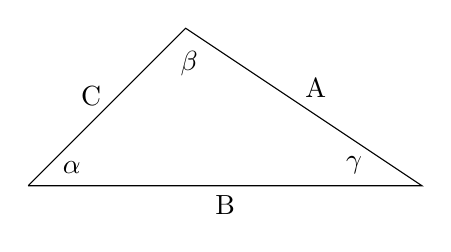
\begin{tikzpicture}
        \draw (0,0) coordinate (a) 
        -- node[pos=0.5, below]{B}(5,0) coordinate (b) 
        -- node[pos=0.45, above=0.1cm]{A}(2,2)  coordinate (c) 
        -- node[pos=0.6, above=0.1cm]{C}(a)
        pic["$\alpha$", angle radius=1cm]{angle=b--a--c}
        pic["$\beta$", angle radius=0.75cm]{angle=a--c--b}
        pic["$\gamma$", angle radius=1.5cm]{angle=c--b--a};
    \end{tikzpicture}
\end{center}

\subsection*{\underline{Proof}:}

Imagine we draw a line from the $\beta$ corner down to the B side length to make a right triangle and label the new line $X$.\\
\begin{center}
    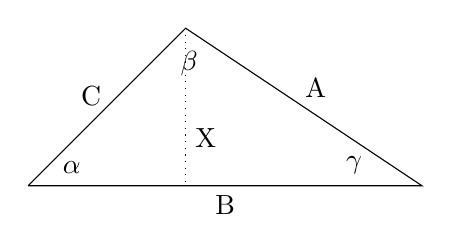
\begin{tikzpicture}
        \draw (0,0) coordinate (a) 
        -- node[pos=0.5, below]{B}(5,0) coordinate (b) 
        -- node[pos=0.45, above=0.1cm]{A}(2,2)  coordinate (c) 
        -- node[pos=0.6, above=0.1cm]{C}(a)
        pic["$\alpha$", angle radius=1cm]{angle=b--a--c}
        pic["$\beta$", angle radius=0.75cm]{angle=a--c--b}
        pic["$\gamma$", angle radius=1.5cm]{angle=c--b--a};
        \draw[dotted] (c) -- node[pos=0.7, right]{X}(2,0);
    \end{tikzpicture}
\end{center}
Since we have created two right triangles that share a length $X$ we can sove for $X$ with two different equations:
\begin{center}
    $sin(\alpha)=\frac{X}{C}$ and $sin(\gamma)=\frac{X}{A}$\\
    $C*sin(\alpha)=X$ and $A*sin(\gamma)=X$\\
    $C*sin(\alpha)=X$ and $A*sin(\gamma)=X$\\
\end{center}
If we set the equations equal to each other we can gain most of the relationship:
\begin{center}
    $C*sin(\alpha) = A*sin(\gamma)$\\
    $C*\frac{sin(\alpha)}{A} = sin(\gamma)$\\
    $\frac{sin(\alpha)}{A} = \frac{sin(\gamma)}{C}$\\
\end{center}
In these steps we have draw a vertical line stemming from one corner of the triangle to make two right triangles incorporating the other two corners. Doing this we have shown that the $sine$ of the angle each corner produces over the side length opposite to each corner is equal.\\
\\
With this proven we can assert that not only does $\frac{sin(\alpha)}{A} = \frac{sin(\gamma)}{C}$, but $\frac{sin(\alpha)}{A} = \frac{sin(\beta)}{B}$ which we could prove with a line stemming from the $\gamma$ corner to side length C.\\
\\
Therefore, by transitive property, if $\frac{sin(\alpha)}{A} = \frac{sin(\gamma)}{C}$ and $\frac{sin(\alpha)}{A} = \frac{sin(\beta)}{B}$, then $\frac{sin(\alpha)}{A} = \frac{sin(\beta)}{B} = \frac{sin(\gamma)}{C}$.\\
\begin{flushright}
    
\begin{tikzpicture}
        \filldraw[fill=black](0,0) rectangle (0.3,0.3);
    \end{tikzpicture}
\end{flushright}

\end{document}